\documentclass[journal,onecolumn, draftclsnofoot, 12pt]{IEEEtran}
\usepackage[margin=1in]{geometry}
\usepackage[utf8]{inputenc}
\usepackage{graphicx}
\usepackage{times}
\usepackage{amsmath,amsfonts,amssymb,amsthm,commath,dsfont,enumitem}
\usepackage[colorlinks,urlcolor=blue,citecolor=blue]{hyperref}
\usepackage{xcolor}

\usepackage{listings}
\usepackage{todonotes}
\usepackage[T1]{fontenc}
\lstset{language=Python,
basicstyle=\fontfamily{fvm}\selectfont\footnotesize}

% macros adapted from matus & djhsu
\def\ddefloop#1{\ifx\ddefloop#1\else\ddef{#1}\expandafter\ddefloop\fi}
\def\ddef#1{\expandafter\def\csname bb#1\endcsname{\ensuremath{\mathbb{#1}}}}
\ddefloop ABCDEFGHIJKLMNOPQRSTUVWXYZ\ddefloop
\def\ddef#1{\expandafter\def\csname b#1\endcsname{\ensuremath{\mathbf{#1}}}}
\ddefloop ABCDEFGHIJKLMNOPQRSTUVWXYZ\ddefloop
\def\ddef#1{\expandafter\def\csname c#1\endcsname{\ensuremath{\mathcal{#1}}}}
\ddefloop ABCDEFGHIJKLMNOPQRSTUVWXYZ\ddefloop

\DeclareMathOperator*{\argmin}{arg\,min}
\DeclareMathOperator*{\argmax}{arg\,max}
\DeclareMathOperator*{\softmax}{softmax}

\newenvironment{Q}{\item}{\phantom{s}}
\newenvironment{Solution}{\color{blue}\begin{enumerate}}{\end{enumerate}}
%\newcommand{\todo}[1]{\textbf{\color{red} [TODO] #1}}

\title{ECE420 Project Proposal\\ Let Him Sing }
\author{Ethan Zhou, Eric Tang \\
\{yz69, leweit2\} @ illinois.edu}

\begin{document}
\maketitle
\section{Introduction}
Inspired by "South Park" season 18 episode 4, where Randy, the protagonist's dad, assumes the identity of famous female singer Lorde using auto-tune. The goal for this project is to implement an auto-tune app that takes in any songs with vocals, and audio of the user singing, separates the vocals from the songs, and remaps the user's voice into the song with temporal and pitch correction applied. The Repeating Pattern Extraction Technique (REPET) will be used for music/voice separation, and TD-PSOLA will be used for voice synthesis.

\section{Overview of the algorithm}
The primary algorithm used in this project would be the Repeating Pattern Extraction Technique (REPET). It achieves voice/music separation. The algorithm is discussed in detail in the paper: "REpeating Pattern Extraction Technique: A Simple Method for Music/Voice Separation" \cite{rafii2012repeating}.

\vspace{0.5cm}
\begin{itemize}
    \item \textbf{Step 1: Identifying repeating pattern} 
\end{itemize}
\begin{description}
   Repeating Periods could be found by using auto-correlation. Given a mixture signal x, first calculate its STFT X, using half-overlapping hamming windows of N samples, then derive the magnitude spectro gram V by taking abs(X). To emphasize the appearance of peaks of periodicity in B, $V^2$ is used. The overall acoustic self-similarity b of x is obtained by averaging the rows of B. As shown in the following equations.
\end{description}



         \[B(i,j) = \frac{1}{m-j+1}\sum_{k=1}^{m-j+1} V(i,k)^2V(i,k + j - 1)^2 \]
         \[b(j)=\frac{1}{n}\sum_{i=1}^{n}B(i,j)\] \[then : b(j)=\frac{b(j)}{b(1)}\]
         for \(i= 1 \dots n\)(frequency)where \(n = \frac{N}{2} + 1\)
         \centering
         \\
         for \(j= 1 \dots m\)(lag) where \(m\) = number of time frames
         \centering
         \\

\begin{description}
   A simple procedure for automatically estimating the repeating period p. The idea is to find which period in the beat spectrum has the highest mean accumulated energy over its integer multiples. For each possible period j in b, we check if its integer multiples i correspond to the highest peaks in their respective neighborhoods, where Delta is a variable distance parameter, the function of j. At the end, we minus the mean of the given neighborhood to filter any possible noisy background.
\end{description}
         \textbf{for} each possible period j in the first 1/3 of b \textbf{do}
         \\
        \\
        \Delta \leftarrow [3j/4], I \leftarrow 0
        \\
         \textbf{for} each possible integer multiple i of j in b \textbf{do}
         \\
         h \leftarrow $argmax$ b(k)   (k \in [i-\Delta , i+\Delta])
         \\
         \textbf{if} h = $argmax$ b(k) \textbf{then}
         \\
         I \leftarrow I + b(h) - avg(b(k))
         \\
         \textbf{end if}
         \\
         \textbf{end for}
         \\
         J(i) \leftarrow I/[l/j]
         \\
         \textbf{end for}
         \\
         p \leftarrow $argmax_{j}$ J(j) 

\vspace{0.5cm}
\begin{itemize}
    \item \textbf{Step 2: Repeating Segment Modeling} 
\end{itemize}
\begin{description}
   Once the repeating period p is estimated from the beat spectrum b, we evenly time-segment the spectrogram V in to r segments of length p. Define the repeating segment model S as the element wise median of the r segments.   
\end{description}

    \[S(i,l) = \underset{k=1,,,r}{\mathrm{median}} \{V(i,l+(k-1))\}\]
    for \(i= 1 \dots n\)(frequency) and \(l = 1 \dots p\)(time)
    \centering
    \\
    define \(p\) = period length, \(r\) = number of segments
    \centering
    


\vspace{0.5cm}
\begin{itemize}
    \item \textbf{Step 3: Repeating Patterns Extraction} 
\end{itemize}
\begin{description}
   Once the repeating segment model S is calculated, it can be used to derive a repeating spectrogram model W, by taking the element wise minimum between S and each of the r segments of the spectrogram V. 
\end{description}


    \[W(i,l+(k-1)p) = \min{S(i,l),V(i,l+(k-1)p)}\]
    for \(i = 1 \dots n, l = 1 \dots p\) and \(k = 1 \dots r\)

\begin{description}
   Once the repeating spectrogram model W is calculated, a soft time-drequency mask M could be derived by normalizing W by V element-wise. The idea is time-frequency bins that are likely to repeat at period p in V will have values near 1 in M and will be weighted toward the repeating background and time-frequency bins that are not likely to repeat at period p in V would have values near 0 in M .
\end{description}
    \[M(i,j) = \frac{W(i,j)}{V(i,j)}\]
    for \ i =1 \dots n (frequency) and j = 1 \dots m (time)






\begin{figure}[ht]
\centering
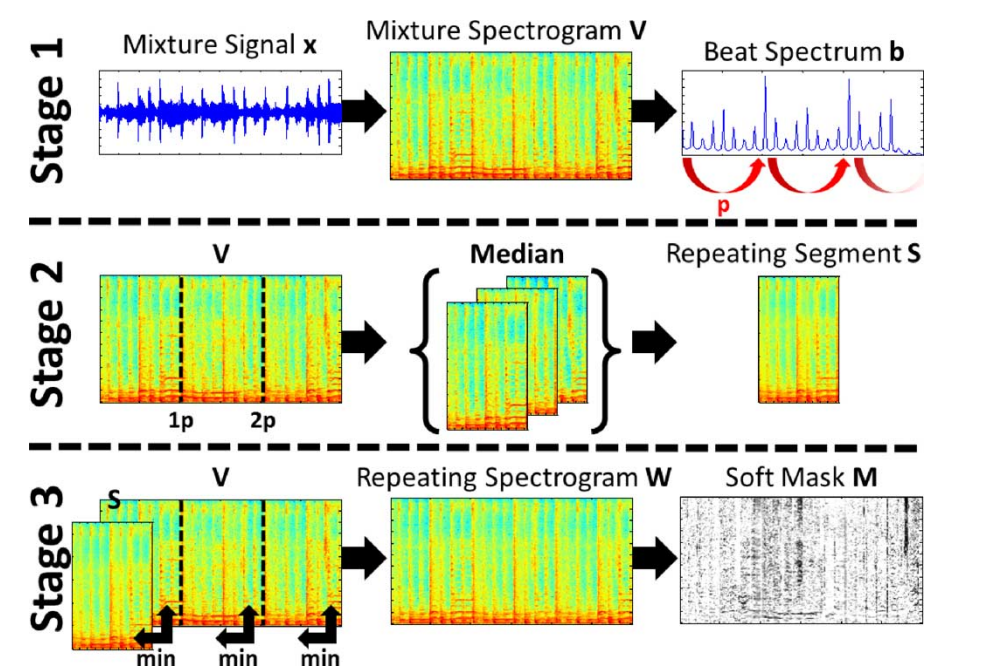
\includegraphics[width=0.7\textwidth]{Figure1.png}
    \caption{ Overview of the  Algorithm  } 

\end{figure}

\vspace{0.5cm}
\begin{itemize}
    \item \textbf{Step 4: Detecting Voiced components} 
\end{itemize}
\begin{description}
   We will determine whether a period of both user input and the separated voice track. We will use pauses in voiced components to segment the entire soundtrack into sentences, which then allows us to apply temporal correction by directly stretching/compressing user input. Assuming the correction needed is not very large, thus the distortion of sounds produced by the vocal track is not significant.
\end{description}

\vspace{0.5cm}
\begin{itemize}
    \item \textbf{Step 5: Pitch detection} 
\end{itemize}
\begin{description}
   we first segment each sentence into 40ms chunks, then apply pitch detection via auto-correlation. This will give us the spectrogram of the original voice in the song, and user input.
\end{description}

\vspace{0.5cm}
\begin{itemize}
    \item \textbf{Step 7: Pitch Synthesis} 
\end{itemize}
\begin{description}
   We will map the user input to the original soundtrack by TD-PSOLA
\end{description}




\section{Plan for testing and validation}
\begin{itemize}
    \item To demonstrate this algorithm work, we can sing into the microphone and listen to the output
    \item The inputs we will be using is a pre-existing song, and the microphone on android device to record user singing. 
    \item The output will be the final pitch/temporal corrected song. The metric would be the pitch correction accuracy, which would be measured by the deviation of the target and corrected spectrogram.
    \item We will start with shorter and simpler soundtracks to test the voice separation effectiveness and work our way to more complex and longer soundtracks and test the accuracy of the entire system.
    
\end{itemize}

\section{Contribution}
\begin{itemize}
    \item Ethan Zhou: task A, C, E, F
    \item Eric Tang: task B, D, E, F
\end{itemize}


\begin{table}[h]
\small
    \centering
    \begin{tabular}{|p{1.5in}|p{1.5in}|}
        \hline
        \textbf{Contents} & \textbf{Number} \\
         \hline
        task A &  Implement the voice/music separation algorithm in Python \\
        \hline
        task B &  Implement the remaining elements in Python \\
        \hline
        task C &  Implement the voice/music separation algorithm in C++ \\
        \hline
        task D &  Implement the remaining elements in C++ \\
        \hline
        task E &  Android integration of functions and UI \\
        \hline
        task F &  Project video for extra credit (optional) \\
        \hline
         
    \end{tabular}
    \vspace{0.1in}
    \caption{Tasks and allocations}
    \label{tab:table}
\end{table}
 


 
\bibliographystyle{IEEEtran}
\bibliography{ref}

\end{document}
